\chapter{Implementación física de la FPU del ASP y bloques de memoria}

Se describe en este capítulo el proceso completo de back end, usando como ejemplo la FPU descrita en \cite{Francis2016, concapan}, y la incorporacion de un macro de SRAM, desarrollado con la herramienta de generación de memorias provista por el kit de ARM. 

Con respectoa la FPU, se partió del RTL, haciendo una integración jerárquica. La primera corresponde a síntesis lógica de los dos módulos principales (suma y multiplicación) y la evaluación post síntesis de las mismas, la segunda etapa consiste en la integración física de cada unidad por separado, y posteriormente se efectúa una evaluación post implementación. Por último se integra el siguiente nivel en la jerarquía, que sirve como módulo principal que instancia los otros dos módulos mencionados.

Tanto la síntesis lógica como física siguen el proceso descrito en el capítulo anterior, según las secciones \ref{sec:syn_s} y \ref{sec:phy_s} respectivamente. Las restricciones consideradas para el proceso de front end y consecuentemente los scripts para la síntesis lógica son las mismas que las mostradas en la sección \ref{s_sec:const}, por lo que no se redundará en esos aspectos.

Respecto a la síntesis física, se consideraron las siguientes configuraciones para la síntesis del árbol de reloj:

\begin{itemize}
\item Inserción de celdas frontera cercanas a los puertos de reloj para el diseño basado en jerarquía de bloques.
\item \texttt{OCV\_Clustering}, para mejorar la distribución del reloj a través de ramas de registros. 
\item Permitir la re-ubicación y el re-dimensionamiento de las compuertas y búfers para optimizar la síntesis del árbol de reloj.
\end{itemize}

Las reglas de antena tienen los siguientes atributos:
\begin{itemize}
\item Modalidad de protección de diodo limitada.
\item Una razón de metal de 150, un tamaño de compuerta por defecto de 0,1, con una protección por defecto de 0,5.
\item Un radio de corte de 20, y una razón de diodo comprendida en el siguiente vector \{0,09 0 123 16880\} para los metales de las capas bajas(cuatro primeras capas de metal), mientras que para las vías de estos primeros cuatro metales el vector sería \{0,09 0 110 500\}
\end{itemize}

Respecto al enrutado global no hay una serie de restricciones o configuraciones específicas para que la herramienta logre enrutar de forma adecuada toda la celda. Este proceso es algo engorroso, y responde más a una metodología iterativa y de optimización selectiva de acuerdo con los resultados que se van dando al trabajar con el trazado del diseño. Sin embargo, se especifican parámetros como la reducción del efecto de diafonía ( \textit{Crosstalk}) para que en el enrutado se eviten colocar cables largos adyacentes a rieles paralelos, y tener un esfuerzo alto al controlar la ejecución de enrutamiento detallado e iterativo para determinar si el DRC diverge.

En relación con los \textit{IP Cores} de las memorias, se efectuó un flujo equivalente. No obstante los \textit{IP Cores} no pueden optimizarse ni trabajarse con mucho detalle, pues precisamente son cajas negras que buscan la protección de la propiedad itelectual. Así que para corroborar que la implementación de estos bloques fuese correcta se evaluaron diseños que hacen de envoltorio (wrapper) para estas celdas, en inglés a esta técnica se le conoce como \textit{"Wrapper"} y en esencia consiste en crear un código que instancie \textit{IP Core} y se sintetiza con base en él. Esto no es estrictamente necesario ya que el código que genera la herramienta tiene una estructura GLN y permite hacer simulaciones post síntesis, si se generan los archivos \texttt{*.sdf} mediante un \textit{script} de PERL. La alternativa del \textit{wrapper} permite usar el \textit{IP Core} como una instancia y usar la metodología que ha sido definida para el flujo.

\section{Resultados de la síntesis lógica de la FPU}
\label{sec:fpu_syn_result}
En esta sección únicamente serán presentados los resultados obtenidos de la síntesis todo el bloque de la FPU pues incluir los resultados previos de los módulos de suma/resta y multiplicación sería redundante.

En la figura \ref{fig:fpu_cell} se muestra el resultado de la implementación de la unidad aritmética de punto flotante en la tecnología IBM 0.13 según el flujo de diseño establecido en este trabajo.

\begin{figure}[h]
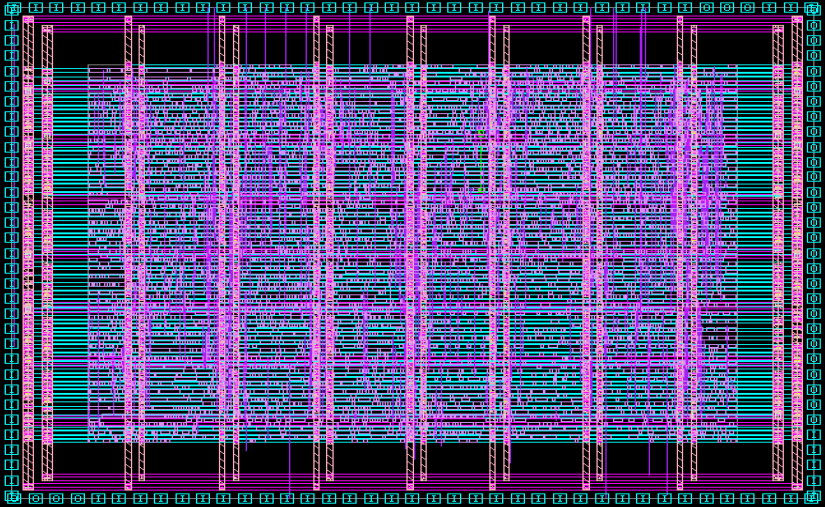
\includegraphics[width=\textwidth]{fpu_cell.png}
\centering
\caption{Foto captura del layout de la celda física generada para la unidad de punto flotante del ASP}
\label{fig:fpu_cell}
\end{figure}

\subsection{Reportes de síntesis lógica}
\label{s_sec:fpu_syn_report}

Al igual que en el capítulo anterior en este apartado se ofrece un resumen de los reportes más relevantes que ofrece la herramienta para evaluar el desempeño del diseño en términos de área, consumo de energía y sincronización de señales. Presentar datos sobre las celdas y los puertos  ofrecen información útil para efectuar un analisis más conciente sobre la administración de los recursos de la tecnología; sin embargo, esta por fuera del enfoque de este trabajo.\\

\newpage
\begin{table}[ht]
\centering
\label{tab:fpu_pwr_tb}
\caption{Resumen del reporte de potencia de la FPU post síntesis lógica}
\begin{tabular}{||l | c | c | c | c | c |}
\hline
\hline
Group & Internal & Switching  & Leakage & Total & \% Attrs \\
\hline
io\_pad & 0.0000 & 0.0000 & 0.0000 & 0.0000 & 0.00\% \\
\hline
memory & 0.0000 & 0.0000 & 0.0000 & 0.0000 & 0.00\% \\
\hline
black\_box & 0.0000 & 0.0000 & 0.0000 & 0.0000 & 0.00\% \\
\hline
clock\_network & 0.0000 & 0.0000 & 0.0000 & 0.0000 & 0.00\% \\
\hline
register & 1.2521 & 0.1130 & 2.4467e+04 & 1.3651 & 60.92\%\\
\hline
sequential  & 0.0000 & 0.0000 & 0.0000 & 0.0000 & 0.00\% \\
\hline
combinational & 0.2211 & 0.6546 & 5.0897e+04 & 0.8757 & 39.08\% \\
\hline
Total &  1.4732 mW & 0.7675 mW & 75.364e+04 nW & 2.2408 mW & 100\%\\
\hline
\hline
\end{tabular}
\end{table}

\begin{lstlisting}[caption={Reporte de área de la unidad de punto flotante de ASP post síntesis lógica.} \label{lst:fpu_area_report}, frame={single}]
****************************************
Report : area
Design : FloatingPointUnit
Version: L-2016.03-SP3
Date   : Tue Jan  3 18:53:58 2017
****************************************

	Library(s) Used: scx3_cmos8rf_lpvt_tt_1p2v_25c

          Number of ports:                          355
          Number of nets:                          5590
          Number of cells:                         4909
          Number of combinational cells:           4227
          Number of sequential cells:               680
          Number of macros/black boxes:               0
          Number of buf/inv:                        792
          Number of references:                      54

          Combinational area:              41843.520412
          Buf/Inv area:                     3906.720098
          Noncombinational area:           20897.279408
          Macro/Black Box area:                0.000000
          Net Interconnect area:          588843.014587

          Total cell area:                 62740.799820
          Total area:                     651583.814407
\end{lstlisting}

\newpage

\begin{lstlisting}[caption={Reporte de sincronía de la FPU post síntesis lógica.} \label{lst:fpu_timing_report}, frame={single},basicstyle=\small]
****************************************
Report : timing -path full -delay max -max_paths 1
Design : FloatingPointUnit Version: L-2016.03-SP3
****************************************
		Path Group: clk | Path Type: max
	
    Startpoint:FPU_Multiplication_Function/Operands_load_reg/
    XMRegister/Q_reg[21](rising edge-triggered flip-flop 
    clocked by CLK)
    Endpoint:FPU_Multiplication_Function/Sgf_operation/SgfM_mul_0.left/
    pdt_int_reg[23](rising edge-triggered flip-flop clocked by CLK)
  -------------------------------------------------------------------
  Des/Clust/Port     Wire Load Model       	Library
  FloatingPointUnit	ibm13_wl10     scx3_cmos8rf_lpvt_tt_1p2v_25c
  -------------------------------------------------------------------
  Point							Incr	Path
  clock CLK (rise edge)					0.00	0.00
  clock network delay (ideal)				1.00	1.00
  FPU_Multiplication_Function/Operands_load_reg/
  XMRegister/Q_reg[21]/CK (DFFRX4TS)			0.00	1.00 r
  FPU_Multiplication_Function/Operands_load_reg/
  XMRegister/Q_reg[21]/QN (DFFRX4TS)			1.18	2.18 r
  FPU_Multiplication_Function/U856/Y(INVX2TS)		0.27	2.45 f
  FPU_Multiplication_Function/U1080/Y(CLKXOR2X2TS)	0.63	3.08 f
  FPU_Multiplication_Function/U524/Y (INVX2TS)		0.46	3.54 r
  FPU_Multiplication_Function/U1071/Y (AND2X2TS)	0.48	4.02 r
  FPU_Multiplication_Function/U554/Y (INVX3TS)		0.25	4.27 f
  FPU_Multiplication_Function/U2192/Y (OAI22X1TS)	0.39	4.66 r
  FPU_Multiplication_Function/U2193/S (CMPR32X2TS)	0.75	5.42 f
  FPU_Multiplication_Function/mult_x_22/U195/
  S(CMPR42X2TS)						0.98	6.39 f
  FPU_Multiplication_Function/mult_x_22/U194/
  S(CMPR42X1TS)						1.19	7.58 f
  FPU_Multiplication_Function/U2107/Y(NAND2X1TS)	0.59	8.17 r
  FPU_Multiplication_Function/U2109/Y(OAI21X1TS)	0.51	8.68 f
  FPU_Multiplication_Function/U2110/Y(AOI21X2TS)	0.33	9.02 r
  FPU_Multiplication_Function/U2111/Y(OAI21X4TS)	0.24	9.26 f
  FPU_Multiplication_Function/U2121/Y(AOI21X4TS)	0.29	9.55 r
  FPU_Multiplication_Function/U726/Y(OAI21X4TS)		0.22	9.77 f
  FPU_Multiplication_Function/U725/Y(AOI21X2TS)		0.29	10.06 r
  FPU_Multiplication_Function/U1062/Y(XOR2X2TS)		0.28	10.34 r
  FPU_Multiplication_Function/Sgf_operation/
  SgfM_mul_0.left/pdt_int_reg[23]/D(DFFQX1TS)		0.00	10.34 r
  
  data arrival time						10.34
  
  clock CLK (rise edge)					10.00	10.00
  clock network delay (ideal)				1.00	11.00
  clock uncertainty					-0.50	10.50
  FPU_Multiplication_Function/Sgf_operation/
  SgfM_mul_0.left/pdt_int_reg[23]/CK(DFFQX1TS)		0.00	10.50 r
  library setup time					-0.16	10.34
  data required time						10.34
  -------------------------------------------------------------------
  data required time						10.34
  data arrival time						-10.34
  -------------------------------------------------------------------
  slack (MET)							0.00
  -------------------------------------------------------------------
  
  Startpoint:FPU_Add_Subtract_Function/Oper_Start_in_module/
  ASRegister/Q_reg[0](rising edge-triggered flip-flop 
  clocked by clk)
  Endpoint:FPU_Add_Subtract_Function/Add_Subt_Sgf_module/
  Add_overflow_Result/Q_reg[0]
  (rising edge-triggered flip-flop clocked by clk)
    
  -------------------------------------------------------------------
  Des/Clust/Port     Wire Load Model       	Library
  FloatingPointUnit	ibm13_wl10     scx3_cmos8rf_lpvt_tt_1p2v_25c
  -------------------------------------------------------------------
  Point							Incr	Path
  clock CLK (rise edge)					0.00	0.00
  clock network delay (ideal)				1.00	1.00
  FPU_Add_Subtract_Function/Oper_Start_in_module/
  ASRegister/Q_reg[0]/CK (DFFRX1TS)			0.00	1.00 r
  FPU_Add_Subtract_Function/Oper_Start_in_module/
  ASRegister/Q_reg[0]/Q (DFFRX1TS)			1.17	2.17 f
  FPU_Add_Subtract_Function/U1634/Y (CLKXOR2X4TS)	0.60	2.77 f
  FPU_Add_Subtract_Function/U1102/Y (XOR2X2TS)		0.40	3.17 r
  FPU_Add_Subtract_Function/U1130/Y (NAND2X4TS)		0.43    3.59 f
  FPU_Add_Subtract_Function/U1835/Y (INVX4TS)		0.46	4.05 r
  FPU_Add_Subtract_Function/U1839/Y (XOR2X1TS)		0.68	4.73 r
  FPU_Add_Subtract_Function/U1848/Y (INVX2TS)		0.39	5.11 f
  FPU_Add_Subtract_Function/U1849/Y (NOR2X1TS)		0.61	5.72 r
  FPU_Add_Subtract_Function/U1852/Y (AOI21X2TS)		0.50	6.23 f
  FPU_Add_Subtract_Function/U871/Y (OAI21X2TS)		0.43	6.65 r
  FPU_Add_Subtract_Function/U1436/Y (AOI21X2TS)		0.38	7.04 f
  FPU_Add_Subtract_Function/U1913/Y (OAI21X4TS)		0.31	7.34 r
  FPU_Add_Subtract_Function/U1917/Y (AOI21X4TS)		0.22	7.57 f
  FPU_Add_Subtract_Function/U1921/Y (OAI21X4TS)		0.27	7.83 r
  FPU_Add_Subtract_Function/U1925/Y (AOI21X4TS)		0.22	8.06 f
  FPU_Add_Subtract_Function/U1929/Y (OAI21X4TS)		0.27	8.32 r
  FPU_Add_Subtract_Function/U1933/Y (AOI21X4TS)		0.22	8.55 f
  FPU_Add_Subtract_Function/U1937/Y (OAI21X4TS)		0.27	8.82 r
  FPU_Add_Subtract_Function/U1941/Y (AOI21X4TS)		0.22	9.04 f
  FPU_Add_Subtract_Function/U1945/Y (OAI21X4TS)		0.25	9.29 r
  FPU_Add_Subtract_Function/U1962/Y (AOI21X2TS)		0.21	9.50 f
  FPU_Add_Subtract_Function/U895/Y (XOR2X2TS)		0.28	9.78 r
  FPU_Add_Subtract_Function/U1963/Y (CLKMX2X2TS)	0.41	10.20 r
  FPU_Add_Subtract_Function/Add_Subt_Sgf_module/
  Add_overflow_Result/Q_reg[0]/D (DFFRX2TS)		0.00	10.20 r
  
  data arrival time						10.20

  clock clk (rise edge)					10.00	10.00
  clock network delay (ideal)				1.00	11.00
  clock uncertainty					-0.50	10.50
  FPU_Add_Subtract_Function/Add_Subt_Sgf_module/
  Add_overflow_Result/Q_reg[0]/CK (DFFRX2TS)		0.00	10.50 r
  library setup time					-0.30	10.20
  data required time						10.20
  -------------------------------------------------------------------
  data required time						10.34
  data arrival time						-10.34
  -------------------------------------------------------------------
  slack (MET)							0.00
  ------------------------------------------------------------------
\end{lstlisting}

\subsection{Reportes de síntesis física}
\begin{table}[ht]
\centering
\label{tab:fpu_pwr_p_tb}
\caption{Resumen del reporte de potencia de la FPU post síntesis física}
\begin{tabular}{||l | c | c | c | c | c |}
\hline
\hline
Group & Internal & Switching  & Leakage & Total & \% Attrs \\
\hline
io\_pad & 0.0000 & 0.0000 & 0.0000 & 0.0000 & 0.00\% \\
\hline
memory & 0.0000 & 0.0000 & 0.0000 & 0.0000 & 0.00\% \\
\hline
black\_box & 0.0000 & 0.0000 & 0.0000 & 0.0000 & 0.00\% \\
\hline
clock\_network & 0.0000 & 0.0000 & 0.0000 & 0.0000 & 0.00\% \\
\hline
register & 1.2530 & 4.7273e-02 & 2.4587e+04 & 1.3003 & 78.51\%\\
\hline
sequential  & 0.0000 & 0.0000 & 0.0000 & 0.0000 & 0.00\% \\
\hline
combinational & 0.1274 & 0.2285 & 5.1105e+04 & 0.3560 & 21.49\% \\
\hline
Total &  1.3804 mW & 0.2758 mW & 75.692e nW & 1.6563 mW & 100\%\\
\hline
\hline
\end{tabular}
\end{table}

\newpage

\begin{lstlisting}[caption={Reporte de área de la unidad de punto flotante de ASP post síntesis lógica.} \label{lst:fpu_area_p_report}, frame={single}]
****************************************
Report : area
Design : FloatingPointUnit
Version: L-2016.03-SP3
Date   : Tue Jan  3 18:53:58 2017
****************************************

	Library(s) Used: scx3_cmos8rf_lpvt_tt_1p2v_25c

          Number of ports:                          144
          Number of nets:                           825
          Number of cells:                          646
          Number of combinational cells:            513
          Number of sequential cells:               131
          Number of macros/black boxes:               0
          Number of buf/inv:                        136
          Number of references:                      63

          Combinational area:              42115.680429
          Buf/Inv area:                     4190.400109
          Noncombinational area:           20897.279408
          Macro/Black Box area:                0.000000
          Net Interconnect area:              undefined
                               (No wire load specified)

          Total cell area:                 63012.959836
          Total area:                 undefined
\end{lstlisting}

\begin{lstlisting}[caption={Reporte de sincronía del microprocesador ASP post síntesis lógica.} \label{lst:fpu_timing_p_report}, frame={single},basicstyle=\small]
**************************************************
Report : timing -path full -delay max -max_paths 1
Design : FloatingPointUnit Version: L-2016.03-SP3
**************************************************
Operating Conditions: tt_1p2v_25c
Library: scx3_cmos8rf_lpvt_tt_1p2v_25c
	Parasitic source    : LPE
	Parasitic mode      : RealRC
	Extraction mode     : MIN_MAX
	Extraction derating : 25/25/25
	
    Startpoint: FPU_Multiplication_Function/Operands_load_reg/
    XMRegister/Q_reg[10](rising edge-triggered flip-flop clocked
    by CLK)
    Endpoint:FPU_Multiplication_Function/Sgf_operation/
    SgfM_mul_0.middle/pdt_int_reg[15](rising edge-triggered 
    flipflop clocked by CLK)
    
    		Path Group: clk | Path Type: max
  -------------------------------------------------------------------
  Des/Clust/Port     Wire Load Model       	Library
  FloatingPointUnit	ibm13_wl10     scx3_cmos8rf_lpvt_tt_1p2v_25c
  -------------------------------------------------------------------
  Point							Incr	Path
  clock CLK (rise edge)					0.00	0.00
  clock network delay (ideal)				1.00	1.00
  FPU_Multiplication_Function/Operands_load_reg/
  XMRegister/Q_reg[10]/CK (DFFRX4TS)			0.00	1.00 r
  FPU_Multiplication_Function/Operands_load_reg/
  XMRegister/Q_reg[10]/QN (DFFRX4TS)			0.88	1.88 f
  FPU_Multiplication_Function/U1092/Y (INVX2TS)		0.44 &	2.32 r
  FPU_Multiplication_Function/U1766/Y (CLKXOR2X2TS)	0.58 &	2.90 f
  FPU_Multiplication_Function/U1767/Y (NOR2X2TS)	0.18 &	3.08 r
  FPU_Multiplication_Function/U1211/Y (XOR2X1TS)	0.49 &	3.56 r
  FPU_Multiplication_Function/U1191/Y (NAND2X6TS)	0.35 &	3.92 f
  FPU_Multiplication_Function/U2505/Y (OAI22X1TS)	0.59 &	4.51 r
  FPU_Multiplication_Function/U1066/S (CMPR32X2TS)	1.06 &	5.57 f
  FPU_Multiplication_Function/DP_OP_110J1_122_5487/
  U307/CO (CMPR42X1TS)					1.15 &	6.73 f
  FPU_Multiplication_Function/DP_OP_110J1_122_5487/
  U303/S (CMPR42X2TS)					1.01 &	7.74 f
  FPU_Multiplication_Function/U1593/Y (NOR2X4TS)	0.18 &	7.92 r
  FPU_Multiplication_Function/U1594/Y (NOR2X2TS)	0.14 &	8.06 f
  FPU_Multiplication_Function/U1596/Y (AOI21X4TS)	0.33 &	8.39 r
  FPU_Multiplication_Function/U408/Y (INVX2TS)		0.22 &	8.61 f
  FPU_Multiplication_Function/U1607/Y (AOI21X1TS)	0.22 &	8.82 r
  FPU_Multiplication_Function/U1051/Y (XOR2X1TS)	0.46 &	9.28 r
  FPU_Multiplication_Function/Sgf_operation/
  SgfM_mul_0.middle/pdt_int_reg[15]/D (DFFQX1TS)	0.00 &	9.28 r
  
  data arrival time						9.28

  clock CLK (rise edge)					10.00	10.00
  clock network delay (ideal)				1.00	11.00
  clock uncertainty					-0.50	10.50
  FPU_Multiplication_Function/Sgf_operation/
  SgfM_mul_0.middle/pdt_int_reg[15]/CK (DFFQX1TS)	0.00	10.50 r
  library setup time					-0.27	10.23
  data required time						10.23
  ------------------------------------------------------------------
  data required time						10.23
  data arrival time						-9.28
  ------------------------------------------------------------------
  slack (MET)							0.94
  
  Startpoint:FPU_Add_Subtract_Function/Oper_Start_in_module/
  YRegister/Q_reg[31](rising edge-triggered flip-flop clocked by clk)
  
  Endpoint:FPU_Add_Subtract_Function/Add_Subt_Sgf_module/
  Add_Subt_Result/Q_reg[24](rising edge-triggered flip-flop
  clocked by clk)
  
  			Path Group: clk | Path Type: max

  Point							Incr	Path
  clock clk (rise edge)					0.00	0.00
  clock network delay (ideal)           		1.00	1.00
  FPU_Add_Subtract_Function/Oper_Start_in_module/
  YRegister/Q_reg[31]/CK (DFFRX1TS)			0.00	1.00 r
  FPU_Add_Subtract_Function/Oper_Start_in_module/
  YRegister/Q_reg[31]/Q (DFFRX1TS)			1.10	2.10 f
  FPU_Add_Subtract_Function/U1634/Y (CLKXOR2X4TS)	0.45 &	2.55 f
  FPU_Add_Subtract_Function/U1102/Y (XOR2X2TS)		0.35 &	2.91 r
  FPU_Add_Subtract_Function/U1130/Y (NAND2X4TS)		0.34 &	3.25 f
  FPU_Add_Subtract_Function/U1129/Y (INVX8TS)		0.17 @  3.42 r
  FPU_Add_Subtract_Function/U1885/Y (XOR2X1TS)		0.43 @	3.85 r
  FPU_Add_Subtract_Function/U1901/Y (NAND2X1TS)		0.43 &	4.28 f
  FPU_Add_Subtract_Function/U880/Y (OAI21XLTS)		0.45 &	4.73 r
  FPU_Add_Subtract_Function/U1903/Y (AOI21X1TS)		0.25 &	4.98 f
  FPU_Add_Subtract_Function/U1904/Y (OAI21X2TS)		0.15 &	5.13 r
  FPU_Add_Subtract_Function/U1436/Y (AOI21X2TS)		0.16 &	5.29 f
  FPU_Add_Subtract_Function/U1913/Y (OAI21X4TS)		0.21 &	5.50 r
  FPU_Add_Subtract_Function/U1917/Y (AOI21X4TS)		0.15 &	5.65 f
  FPU_Add_Subtract_Function/U1921/Y (OAI21X4TS)		0.17 &	5.82 r
  FPU_Add_Subtract_Function/U1925/Y (AOI21X4TS)		0.13 &	5.95 f
  FPU_Add_Subtract_Function/U1929/Y (OAI21X1TS)		0.41 &	6.36 r
  FPU_Add_Subtract_Function/U1933/Y (AOI21X4TS)		0.27 &	6.63 f
  FPU_Add_Subtract_Function/U1937/Y (OAI21X1TS)		0.46 &	7.09 r
  FPU_Add_Subtract_Function/U1941/Y (AOI21X4TS)		0.30 &	7.39 f
  FPU_Add_Subtract_Function/U2006/Y (XOR2X1TS)		0.58 &	7.97 r
  FPU_Add_Subtract_Function/U905/Y (CLKMX2X2TS)		0.60 &	8.57 r
  FPU_Add_Subtract_Function/Add_Subt_Sgf_module/
  Add_Subt_Result/Q_reg[24]/D (DFFRX2TS)		0.00 &	8.57 r
  
  data arrival time						8.57

  clock clk (rise edge)					10.00	10.00
  clock network delay (ideal)				1.00	11.00
  clock uncertainty					-0.50	10.50
  FPU_Add_Subtract_Function/Add_Subt_Sgf_module/
  Add_Subt_Result/Q_reg[24]/CK (DFFRX2TS)		0.00	10.50 r
  library setup time					-0.28	10.22
  data required time						10.22
  -----------------------------------------------------------------
  data required time						10.22
  data arrival time						-8.57
  -----------------------------------------------------------------
  slack (MET)							1.65
\end{lstlisting}

\subsection{Reportes del análisis de sincronización estática (STA)}
\begin{lstlisting}[caption={Reporte STA de la FPU. Anotaciones sobre el análisis entre registros y puertos.} \label{lst:fpu_sta_n_report}, frame={single}]
              ****************************************
              Report : timing
                  -path_type full
                  -delay_type max
                  -slack_lesser_than 0.00
                  -max_paths 40
                  -sort_by slack
              Design : FloatingPointUnit
              Version: K-2015.06-SP3-3
              Date   : Mon Feb 13 16:21:27 2017
              ****************************************

              No paths with slack less than 0.00.
\end{lstlisting}


\begin{lstlisting}[caption={Reporte STA de la FPU. Anotaciones sobre el análisis entre registros y puertos.} \label{lst:fpu_sta_report}, frame={single},basicstyle=\small]
****************************************
Report : timing
	-path_type full
	-delay_type max
	-input_pins
	-nets
	-max_paths 1
	-transition_time
	-capacitance
	-sort_by slack
Design : FloatingPointUnit
Version: K-2015.06-SP3-3
Date   : Mon Feb 13 16:21:37 2017
****************************************


	Startpoint:FPU_Multiplication_Function/Operands_load_reg/
	XMRegister/Q_reg[10]
	(rising edge-triggered flip-flop clocked by CLK)
	Endpoint:FPU_Multiplication_Function/Sgf_operation/
	SgfM_mul_0.middle/pdt_int_reg[15]
	(rising edge-triggered flip-flop clocked by CLK)
		
        Path Group: CLK 	Path Type: max

  Point				Fanout	Cap	Trans	Incr	Path
  ----------------------------------------------------------------------
  clock CLK (rise edge)		--	--	0.50	0.00	0.00
  clock network delay (ideal)	--	--	----	1.00	1.00
  Operands_load_reg/XMRegister/
  Q_reg[10]/CK (DFFRX4TS)	--	--	0.00	0.00	1.00 r
  Operands_load_reg/XMRegister/
  Q_reg[10]/QN (DFFRX4TS)	--	--	0.00	0.88 *	1.88 f
  n576 (net)			2	0.01 
  U1092/A (INVX2TS)		--	--	0.00	0.00 *	1.88 f
  U1092/Y (INVX2TS)		--	--	0.00	0.44 *	2.32 r
  n435 (net)			9	0.08	---- 	----	----
  U1766/A (CLKXOR2X2TS)		--	----	0.00	0.00 *	2.32 r
  U1766/Y (CLKXOR2X2TS)		--	----	0.00	0.58 *	2.90 f
  n1110 (net)			2	0.01	----	----	-----
  U1767/B (NOR2X2TS)		--	----	0.00	0.00	*2.90 f
  U1767/Y (NOR2X2TS)		--	----	0.00	0.18 *	3.08 r
  n1108 (net)			1	0.01	----	----	----
  U1211/A (XOR2X1TS)		--	----	0.00	0.00 *	3.08 r
  U1211/Y (XOR2X1TS)		--	----	0.00	0.49 *	3.56 r
  n1116 (net)			1	0.02	----	----	----
  U1191/A (NAND2X6TS)		--	----	0.00	0.00 *	3.56 r
  U1191/Y (NAND2X6TS)		--	----	0.00	0.35 *	3.92 f
  n1906 (net)			10	0.04	----	----	----
  U2505/B0 (OAI22X1TS)		--	----	0.00	0.00 *	3.92 f
  U2505/Y (OAI22X1TS)		--	----	0.00	0.59 *	4.51 r
  n1910 (net)			1	0.02	----	----	---- 
  U1066/B (CMPR32X2TS)		--	----	0.00	0.00 *	4.51 r
  U1066/S (CMPR32X2TS)		--	----	0.00	1.06 *	5.58 f
  DP_OP_110J1_122_5487/n332(net) 1	0.01	----	----	----
  DP_OP_110J1_122_5487/
  U307/B (CMPR42X1TS)		--	----	0.00	0.00 *	5.58 f
  DP_OP_110J1_122_5487/
  U307/CO (CMPR42X1TS)		--	----	0.00	1.15 *	6.73 f
  DP_OP_110J1_122_5487/n329(net) 1	0.01	----	----	----
  DP_OP_110J1_122_5487/U303/
  C (CMPR42X2TS)		--	----	0.00	0.00 *	6.73 f
  DP_OP_110J1_122_5487/U303/
  S (CMPR42X2TS)		--	----	0.00	1.01 *	7.74 f
  DP_OP_110J1_122_5487/n319(net) 2	0.02	----	---- 
  U1593/A (NOR2X4TS)		--	----	0.00	0.00 *	7.74 f
  U1593/Y (NOR2X4TS)		--	----	0.00	0.18 *	7.92 r
  n1671 (net)			3	0.02	----	----	----
  U1594/A (NOR2X2TS)		--	----	0.00	0.00 *	7.92 r
  U1594/Y (NOR2X2TS)		--	----	0.00	0.14 *	8.06 f
  n976 (net)			1	0.01	----	----	---- 
  U1596/A1 (AOI21X4TS)		--	----	0.00	0.00 *	8.06 f
  U1596/Y (AOI21X4TS)		--	----	0.00	0.33 *	8.39 r
  n1104 (net)			2	0.04	----	----	---- 
  U408/A (INVX2TS)		--	----	0.00	0.00 *	8.39 r
  U408/Y (INVX2TS)		--	----	0.00	0.22 *	8.61 f
  n1669 (net)			4	0.01	----	----	---- 
  U1607/A0 (AOI21X1TS)		--	----	0.00	0.00 *	8.61 f
  U1607/Y (AOI21X1TS)		--	----	0.00	0.22 *	8.83 r
  n986 (net)			1	0.00	----	----	---- 
  U1051/A (XOR2X1TS)		--	----	0.00	0.00 *	8.83 r
  U1051/Y (XOR2X1TS)		--	----	0.00	0.46 *	9.28 r
  Sgf_operation/SgfM_mul_0.middle/
  N15(net)			1	0.02	----	----	----
  Sgf_operation/SgfM_mul_0.middle/
  pdt_int_reg[15]/D (DFFQX1TS)	--	----	0.00	0.00 *	9.29 r
  
  data arrival time		--	----	----	----	9.29

  clock CLK (rise edge)		--	----	0.50	10.00	10.00
  clock network delay (ideal)	--	----	----	1.00	11.00
  clock reconvergence pessimism	--	----	----	0.00	11.00
  clock uncertainty		--	----	----	-0.50	10.50
  Sgf_operation/SgfM_mul_0.middle/
  pdt_int_reg[15]/CK (DFFQX1TS)	--	----	-----	-----	10.50 r
  library setup time		--	----	----	-0.27 *	10.23
  data required time		---	----	----	----	10.23
  -----------------------------------------------------------------
  data required time		--	----	----	----	10.23
  data arrival time		--	----	----	----	-9.29
  -----------------------------------------------------------------
  slack (MET)			--	----	----	-----	0.94
  
  Note: All the points starts from FPU_Multiplication_Function/

\end{lstlisting}

\newpage

\subsection{Simulaciones}
\label{s_sec:fpu_sim}
Dado que en esta sección se analiza el comportamiento de módulos matemáticos, que en esencia brindan el resultado de operar dos datos con una función particular (suma, resta o multiplicación, con signo). Conviene usar una estrategia de verificación que tome la unidad bajo prueba y la estimule con vectores de datos leídos desde archivos fuente, y generar un vector de respuesta, con, valga la redundancia, los resultados de operar los elementos de los vectores de estímulo, y guardar este vector en otro archivo. Generar un vector con las respuestas a un estímulo determinado, permite comparar con mayor facilidad si el diseño ejecuta la función para la que fue concebido después del proceso de síntesis.

Dicho lo anterior este apartado se considera más productivo mostrar un análisis gráfico de los resultados de las simulaciones, pero no mediante diagramas de tiempo, si no realizando un contraste entre las respuestas a las distintas simulaciones, aprovechando el hecho de que la estrategia de simulación usada, en el testbench (aportado junto al RTL de la FPU), consiste en estimular el diseño con un vector de datos leídos desde un archivo fuente, y guardando el vector de respuesta en otro archivo de texto. Mediante la herramienta \texttt{Octave} es posible graficar la relación entre los datos.

El testbench para la FPU, ejercita una serie de pruebas para verificar que las funciones de los módulos son correctos, tiene 2 vectores de estímulo, y mediante un bucle se recorren los vectores estimulando el diseño y almacenando el resultado en un vector, en cada iteración. En total se ejecutan unas mil pruebas.

Se muestra el resultado de esas mil pruebas elaborando un gráfico de la siguiente manera: Se presenta 2 figuras con 3 gráficas (figuras \ref{fig:sim_add} y \ref{fig:sim_add} ), con el fin de no realizar demasiada contaminación visual, se les da un offset (desnivel) a los datos correspondientes a las simulaciones post síntesis, para verificar que tan similares son los resultados. El eje horizontal representa el índice de la muestra del vector de resultados, y el eje vertical muestra la magnitud, es decir el valor del resultado.

Como complemento a estas gráficas también se genera otro par de gráficas que muestran que tan desvidados se encuentran los datos de las simulaciones post síntesis respecto a los esperables según la simulación por comportamiento, que se ha tomado como la referencia dorada del diseño, en ausencia a otro modelo de alto nivel para tomar como referencia.

\newpage


\begin{figure}[h]
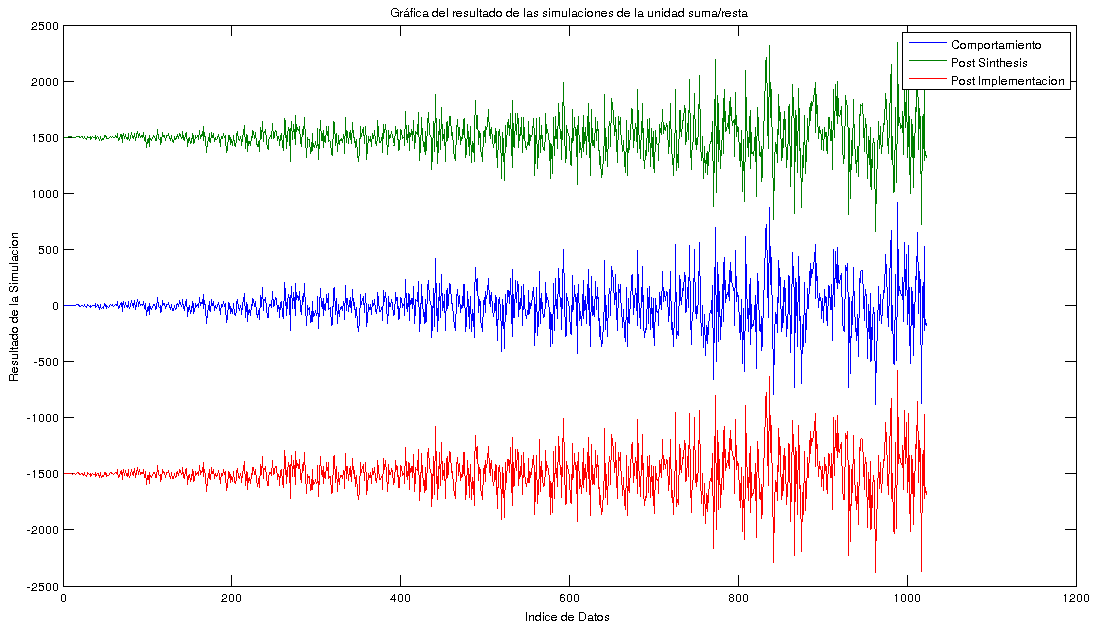
\includegraphics[width=\textwidth,height=8.5cm]{SimulacionADD.png}
\centering
\caption{Gráfico de los resultados de las distintas simulaciones asociadas con el módulo de suma y resta de la FPU. Observar que hay un desface entre los datos, hecho a drede para apreciar mejor la dinámica de las distintas gráficas.}
\label{fig:sim_add}
\end{figure}

\begin{figure}[h]
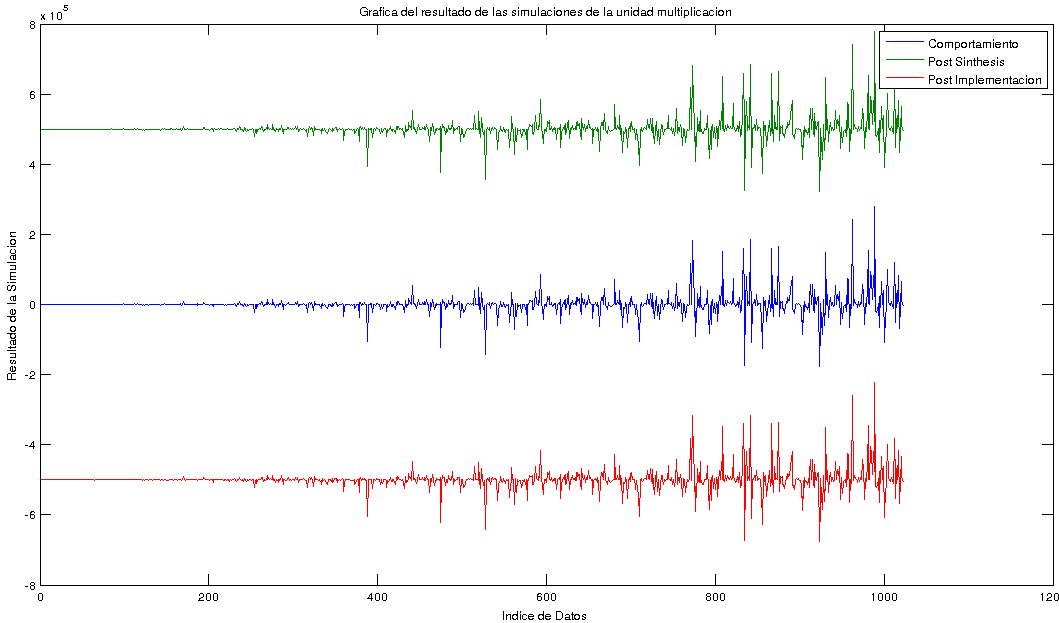
\includegraphics[width=\textwidth,height=9cm]{SimulacionMULT.png}
\centering
\caption{Gráfico de los resultados de las distintos simulaciones asociadas con el módulo de multiplicación con signo de la FPU Observar que hay un desface entre los datos, hecho a drede para apreciar mejor la dinámica de las distintas gráficas.}
\label{fig:sim_mult}
\end{figure}

\newpage


\begin{figure}[h]
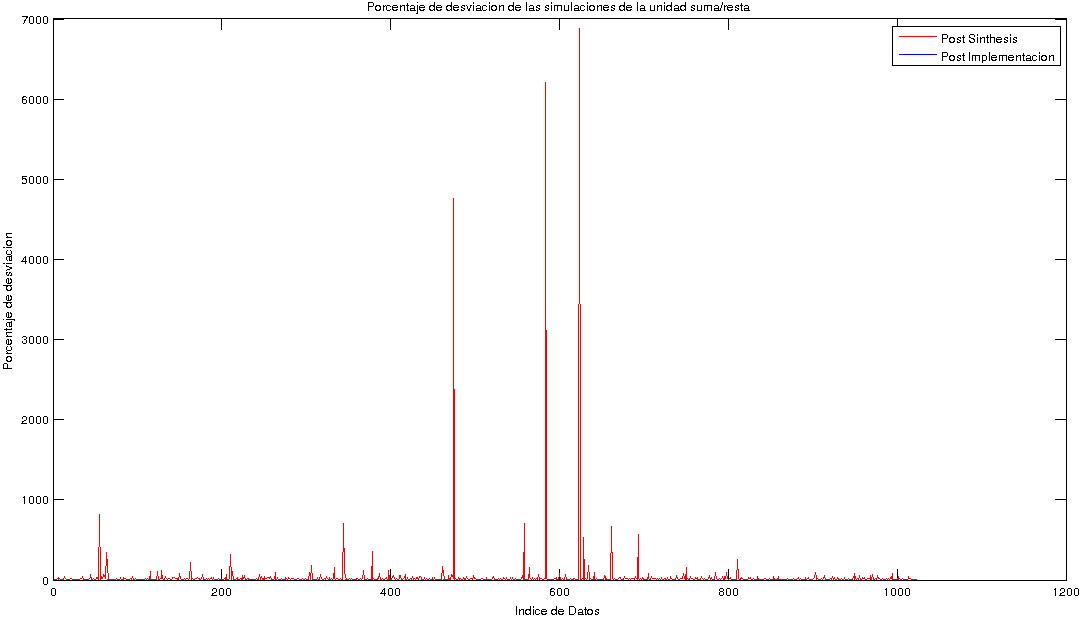
\includegraphics[width=\textwidth,height=8cm]{DesviacionADD.png}
\centering
\caption{Gráfica del porcentaje de desviación, de las simulaciones post síntesis de la unidad de suma y resta de la FPU, respecto a simulación por comportamiento. Se que la simulación post síntesis lógica, presenta algunas incongruencias para ciertos datos, mientras la síntesis física es congruente.}
\label{fig:desv_add}
\end{figure}

\begin{figure}[h]
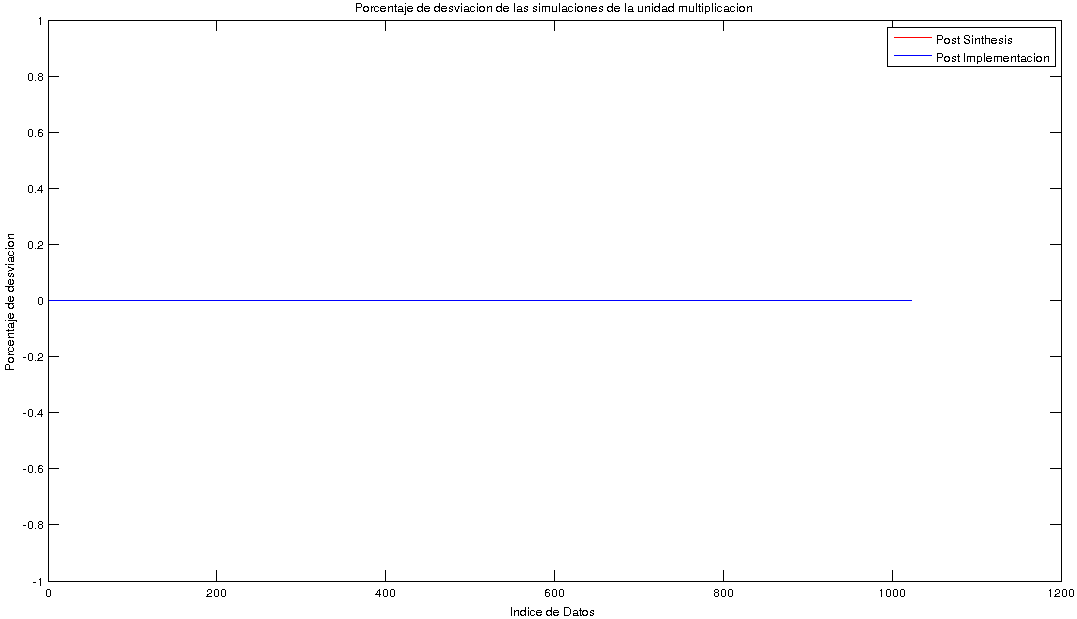
\includegraphics[width=\textwidth,height=8cm]{DesviacionMULT.png}
\centering
\caption{Gŕafica que muestra el porcentaje de desviación, de las simulaciones post síntesis de la unidad de multiplicación de la FPU. Observe que ambas líneas son perfectamente horizontales, lo que indica que la simulaciones post síntesis son consistentes con la de comportamiento}
\label{fig:desv_mult}
\end{figure}

\newpage

\subsection{Análisis de los resultados obtenidos en la implementación de la FPU}

\subsubsection{Potencia}
Comenzando por el análisis de los reportes de potencia post síntesis lógica y post síntesis física (tablas 5.1 y 5.2) se aprecia que respecto a la disipación de energía debido al consumo interno de las celdas y la perdidas por corrientes de fuga (leakage) se mantienen en valores muy similares, pues estos son consecuencias de las celdas propiamente y estos parámetros son difícilmente controlables; sin embargo, la herramienta de IC Compiler de Synopsys permite efectuar una optimización de las pérdidas por corrientes de fuga. Como puede apreciarse este parámetro no varía significativamente. No fue optimizado debido a que su valor es considerablemente bajo y en el proceso (130 nm), no es tan crítico para tomarlo en cuenta, aunque es un posible aspecto a considerar en aplicaciones a escalas más pequeñas y procesos modernos.

Analizando estos reportes observamos que no existe disipación por elementos sequenciales, esto es esperable ya que los módulos aritméticos usados consisten principalmente en lógica combinacional y registros gobernados por una pequeña máquina de estados, que respecto al volumen de los demás elementos no aporta un consumo significativo.

\subsubsection{Área}
Respecto a los reportes de área, códigos: \ref{lst:fpu_area_report} y \ref{lst:fpu_area_p_report}, se observa que en el primero (reporte de síntesis lógica) se tienen una cantidad considerablemente superior de todos los elementos, respecto al segundo reporte que es el de síntesis física. Esto se debe a la metodología de diseño jerárquico, recordando lo expuesto en la sección \ref{sec:phy_s} el diseño jerárquico del layout corresponde a generar una única biblioteca milkyway y cada subdiseño se sintetizará en esta como una celda, posteriormente conforme se avanza en diseños más complejos que usan estas celdas como instancias en el nuevo diseño, siguiendo una metodología \textit{BottomUp}.

El reporte \ref{lst:fpu_area_p_report} (síntesis física) presenta una menor densidad de elementos pues reconoce a los bloques de suma/resta y multiplicación como una celda estándar, en el caso del reporte \ref{lst:fpu_area_report} (síntesis lógica) la herramienta considera todas las dependencias de los módulos mencionados. También se puede observar que el reporte \ref{lst:fpu_area_p_report} (síntesis física) no presenta información sobre el área total que ocupa el diseño, y la información que aporta sólo indica que el diseño presenta una caja negra. No se puede ofrecer una respuesta puntual a esta situación, es probable que esto se deba a una mala configuración de algún parámetro al crear la biblioteca o importar los archivos fuente para generar el layout.

\subsubsection{Sincronía}

Los reportes de síntesis lógica (\ref{lst:fpu_timing_report}) no aportan mucha información relevante pues el modelo de estimación es bastante impreciso debido a la ausencia de un layout formal; sin embargo, sirven como precedente para saber si el diseño abstraído del RTL es coherente con la tecnología y podría ser funcional en la misma. Los reportes de síntesis física (\ref{lst:fpu_timing_p_report}, \ref{lst:fpu_sta_n_report} y \ref{lst:fpu_sta_report}), permiten observar un mejor comportamiento de la propagación de un dato sobre la ruta crítica.

El reporte \ref{lst:fpu_sta_n_report} se encuentra vacío y se debe a que la herramienta no encontró retardos significativos en la propagación de los datos, desde: los puertos de entrada a los registros, de los registros a los puertos de salida o entre registros, por lo tanto estos reportes son despreciables, para este diseño en particular.

Cabe destacar que para el reporte post implementación física (\ref{lst:fpu_timing_p_report}) se analizan 2 rutas críticas tanto para el bloque de suma/resta como para el bloque de multiplicación; sin embargo, el reporte del análisis STA únicamente corresponde al bloque de multiplicación, esto puede deberse a que el módulo de suma implementa una arquitectura optimizada de pipeline \cite{Francis2016}, mientras que el módulo de multiplicación no, es por ello que la herramienta de STA se concentra más en este módulo. En general en todos los casos el \textit{SLACK} es alcanzado, lo cuál indica una correcta implementación.


\subsubsection{Funcionalidad}

En las figuras \ref{fig:sim_add} y \ref{fig:sim_mult} podemos observar el comportamiento del diseño ante una serie de estímulos, en esencia, datos de entrada para verificar si el algoritmo matemático es correcto. Tanto los vectores de estímulo como el vector de respuesta del banco de pruebas (testbench) se encuentran en formato hexadecimal IEEE574. Por lo que se realizó un pequeño script en \texttt{Octave} que convierte del formato IEEE574 a representación decimal estándar.

Dicho lo anterior se grafican los resultados tal y como se explicó en la sección \ref{s_sec:fpu_sim}. Las gráficas permiten dilucidar que tanto los módulos de suma y resta funcionan adecuadamente, pues presentan el mismo patrón que la simulación por comportamiento, la cual se toma como la referencia dorada para evaluar los resultados de la implementación. 

Cabe resaltar la particularidad que se muestra en la figura \ref{fig:desv_add}, en esta figura se muestra una relación porcentual de desviación entre el dato de la referencia dorada y el dato obtenido en la simulación post síntesis, la gráfica correspondiente al resultado post síntesis lógica diverge enormente para algunos estímulos puntuales, ubicados cerca de la mitad del vector de estímulo; sin embargo, la variabilidad de los datos de la simulación post síntesis física no es significativa, lo cual lleva a considerar que hay algún problema en el modelado de la síntesis lógica, probablemente por no definir adecuadamente las restricciones de diseño para el reloj durante el flujo de front end. Dado que las simulaciones post síntesis física y los reportes de sincronía indican que el diseño funciona adecuadamente, puede considerarse que el diseño es correcto.


\section{Integración de los \textit{IP Cores} de memorias SRAM}

Respecto a los \textit{IP Cores}, cabe destacar que se generaron 2 bloques de memoria SRAM de 4000 palabras y 2 palabras con un tamaño de palabra de 32 bits, con el fin de crear un precedente para la posterior integración correcta de los bloques de memoria para el microprocesador ASP. Los bloques fueron definidos con un tamaño arbitrario, considerando que un bloque de 4k es suficiente para la memoria de datos del ASP, y 2k son suficientes para la memoria de programa del ASP. Estas dimensiones se consideran una magnitud significativa para poder demostrar la inclusión de \textit{IP Cores} dentro de un diseño.

La metodología seguida corresponde a la expuesta en la sección \ref{sec:ip_syn}, como se mencionó al inicio de este capítulo la técnica usada para demostrar la correcta generación del \textit{IP Core} es la de crear un wrapper, el cual en esencia es un códito HDL que instancia la celda generada. Luego esta nueva celda (wrapper) se somete al flujo hasta generar un layout, donde aparece una celda estándar correspondiente al \textit{IP Core} generado.

Es posible presentar todos los reportes asociados con la síntesis lógica y física de esta unidad; sin embargo, sería saturar de información redundante este trabajo, por lo que partiendo de la premisa de que la celda generada, debe ser correcta, pues es concebida con las herramientas propias del proveedor de la tecnología, se omite un análisis exhaustivo de esta integración.

El resultado de la integración del bloque \textit{IP Core} correspondiente a la memoria SRAM para datos (4kx32) y el layout del wrapper usado sería el apreciado en la figura \ref{fig:dram_cell}

\begin{figure}[h]
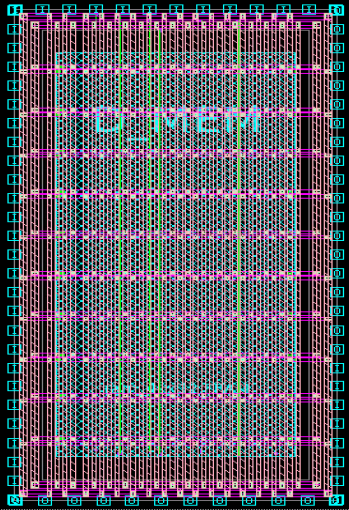
\includegraphics[scale=0.55]{DMEM_cell.png}
\centering
\caption{Foto captura del layout resultante de la impementación del \textit{IP Core} de una memoria SRAM de 4kx32.}
\label{fig:dram_cell}
\end{figure}

Para demostrar la funcionalidad del \textit{IP Core} generado se realiza una pequeña simulación post implementación física. El resultado se aprecia en las figuras \ref{fig:dram_sim_m} y \ref{fig:dram_sim_t}. Puede apreciarse como el dato se escribe (en la dirección ffe) en el primer de reloj, si se presta atención al marcador M1 (línea vertical de color gris) se aprecia entre paréntesis el lapso que existe entre el flanco de la señal de reloj y el cambio en la señal de salida del dato. Este tiempo es distinto para las dos simulaciones siendo mayor en la figura \ref{fig:dram_sim_t} pues considera los retardos máximos del diseño, mientras que la figura \ref{fig:dram_sim_m} muestra el efecto de los retardos mínimos.

\begin{figure}[h]
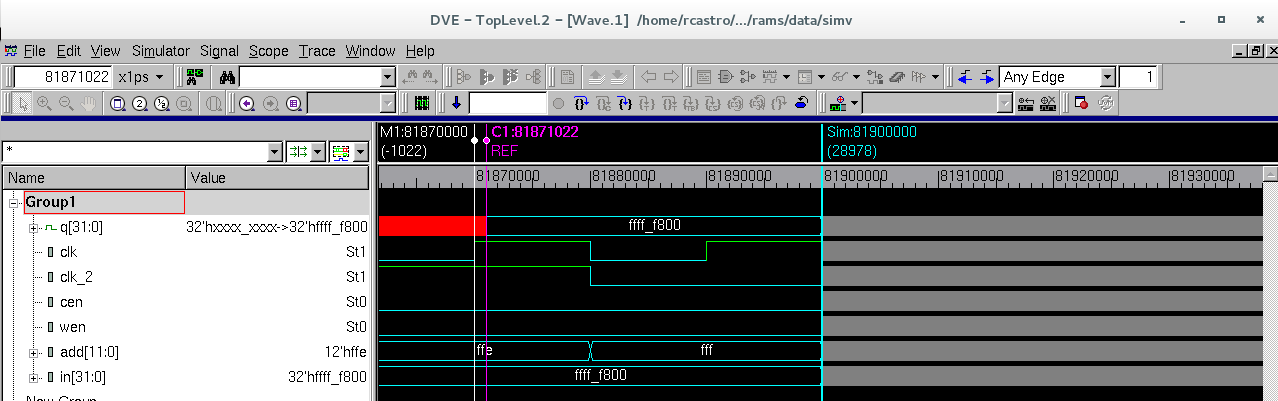
\includegraphics[width=\textwidth]{sim_DMEM_phy_min.png}
\centering
\caption{Simulación post implementación física del \textit{IP Core} para la memoria de datos (4kx32) con el modelo de retardos mínimos}
\label{fig:dram_sim_m}
\end{figure}

\begin{figure}[h]
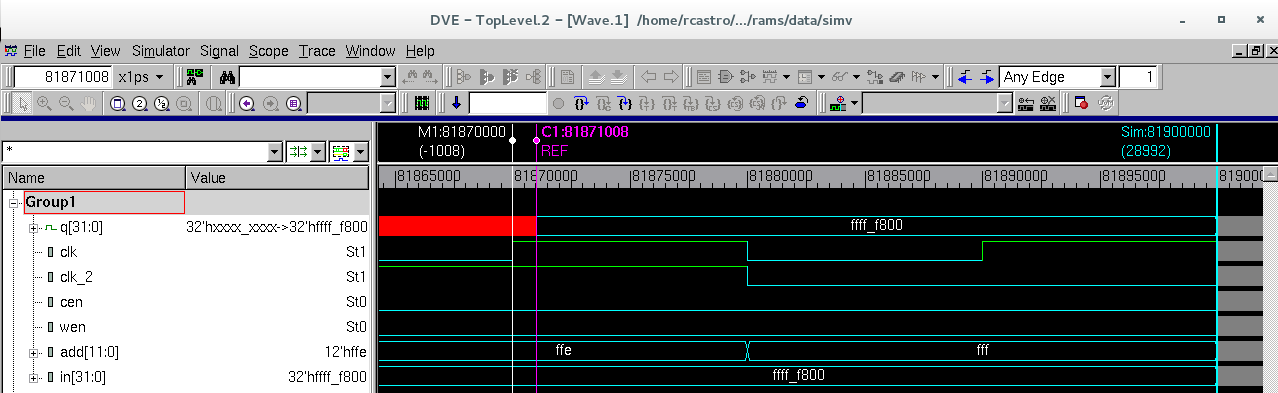
\includegraphics[width=\textwidth]{sim_DMEM_phy_typ.png}
\centering
\caption{Simulación post implementación física del \textit{IP Core} para la memoria de datos (4kx32) con el modelo de retardos típicos}
\label{fig:dram_sim_t}
\end{figure}